\section{Results}
\label{sec:results}
The $10^6$ samples have been post-processed by partitioning the data set in 64 subsets, a subset for each
PDS. 
For each subset/PDS a value of probability and error estimate associated to it have been determined 
(see Section~\ref{sec:plantAnalysisResults}).

Table~\ref{tab:resultsMain} summarizes these findings and it ranks the PDS based on their probability.
First of all, note that 14 out of 64 PDSs were actually generated; i.e., none of the $10^6$ samples 
belong to 50 PDSs.

Secondarily, note that none of the recovery strategies are able to recovery PWR3: its condition at 
the beginning of the accident is the worst among the three units (lost of CST inventory on top of 
SBO condition). From separate calculations, PWR3 could be saved only if EPE3 would be connected
withing the first 50 minutes after SBO condition. Such condition, cannot be met given the boundary
conditions of the accident progression.

PWR1, on the other side, never reach CD condition: this is due to the fact that CST inventory is 
intact (compare to PWR3) and, thus, the time required to reach CD condition is much longer. In addition,
PWR1 can be put in safe condition through several ways (see Section~\ref{sec:testCase}).

PWR2 and the SFPs appear to reach both CD and OK condition. The objective of the analysis is now 
to understand what are the driving factors behind each PDS instead of focusing only on PDS 
probabilities. 

\begin{table}
  \centering
  \begin{tabular}{c|cccccc|ccc}
    \hline
    ID & \multicolumn{6}{c}{PDS} & \multicolumn{3}{c}{Probability}   \\
    \cline{2-10}
         & PWR1 & PWR2 & PWR3 & SFP1 & SFP2 & SFP3 & mean & $5^{th}$ & $95^{th}$     \\
    \hline \hline
      8    & OK   & OK   & \cellcolor[gray]{0.95}CD   & OK   & OK   & OK   & 0.890199555 & 0.889684864 & 0.890713359 \\
      12   & OK   & OK   & \cellcolor[gray]{0.95}CD   & \cellcolor[gray]{0.95}CD   & OK   & OK   & 0.058915971 & 0.058529164 & 0.059303781 \\
      10   & OK   & OK   & \cellcolor[gray]{0.95}CD   & OK   & \cellcolor[gray]{0.95}CD   & OK   & 0.033966983 & 0.033669558 & 0.034265467 \\
      9    & OK   & OK   & \cellcolor[gray]{0.95}CD   & OK   & OK   & \cellcolor[gray]{0.95}CD   & 0.012604994 & 0.012422046 & 0.012789049 \\
      24   & OK   & \cellcolor[gray]{0.95}CD   & \cellcolor[gray]{0.95}CD   & OK   & OK   & OK   & 0.002102999 & 0.002028218 & 0.002178912 \\ 
      13   & OK   & OK   & \cellcolor[gray]{0.95}CD   & \cellcolor[gray]{0.95}CD   & OK   & \cellcolor[gray]{0.95}CD   & 0.001172999 & 0.001117271 & 0.001229862 \\
      14   & OK   & OK   & \cellcolor[gray]{0.95}CD   & \cellcolor[gray]{0.95}CD   & \cellcolor[gray]{0.95}CD   & OK   & 0.000581    & 0.00054194  & 0.000621195 \\    
      11   & OK   & OK   & \cellcolor[gray]{0.95}CD   & OK   & \cellcolor[gray]{0.95}CD   & \cellcolor[gray]{0.95}CD   & 0.000165    & 0.000144457 & 0.00018668  \\     
      26   & OK   & \cellcolor[gray]{0.95}CD   & \cellcolor[gray]{0.95}CD   & OK   & \cellcolor[gray]{0.95}CD   & OK   & 0.000156    & 0.000136041 & 0.000177095 \\
      28   & OK   & \cellcolor[gray]{0.95}CD   & \cellcolor[gray]{0.95}CD   & \cellcolor[gray]{0.95}CD   & OK   & OK   & 0.000111    & 9.43E-05    & 0.000128878 \\
      25   & OK   & \cellcolor[gray]{0.95}CD   & \cellcolor[gray]{0.95}CD   & OK   & OK   & \cellcolor[gray]{0.95}CD   & 1.10E-05    & 6.17E-06    & 1.70E-05    \\ 
     15   & OK   & OK   & \cellcolor[gray]{0.95}CD   & \cellcolor[gray]{0.95}CD   & \cellcolor[gray]{0.95}CD   & \cellcolor[gray]{0.95}CD   & 6.00E-06    & 2.61E-06    & 1.05E-05    \\     
     30   & OK   & \cellcolor[gray]{0.95}CD   & \cellcolor[gray]{0.95}CD   & \cellcolor[gray]{0.95}CD   & \cellcolor[gray]{0.95}CD   & OK   & 5.00E-06    & 1.97E-06    & 9.15E-06    \\         
     29   & OK   & \cellcolor[gray]{0.95}CD   & \cellcolor[gray]{0.95}CD   & \cellcolor[gray]{0.95}CD   & OK   & \cellcolor[gray]{0.95}CD   & 1.00E-06    & 5.13E-08    & 3.00E-06    \\    
    \hline
  \end{tabular}
  \caption{Multi-unit analysis results.}
  \label{tab:resultsMain}
\end{table}

In the next sections, each of the 24 data subsets (i.e, 24 PDs) is analyzed in order to 
discover the input drivers for each PDS. For the majority of them we report the histogram 
of the input variables for that particular 
PDS and compare with the full data set. The comparison is made visually by presenting:
\begin{itemize}
  \item the histogram of a specific variable for the full data set in gray color, and, 
  \item the histogram of the same variable for the PDS subset in a brighter color (i.e., not gray)
\end{itemize}

A summary of the relationships among PDSs pictured in a hierarchical fashion is shown in 
Fig.~\ref{fig:PDSsummary}; this figures also summarizes the most important drivers and the
consequences related to the drivers.

\begin{figure}
    \centering
    \centerline{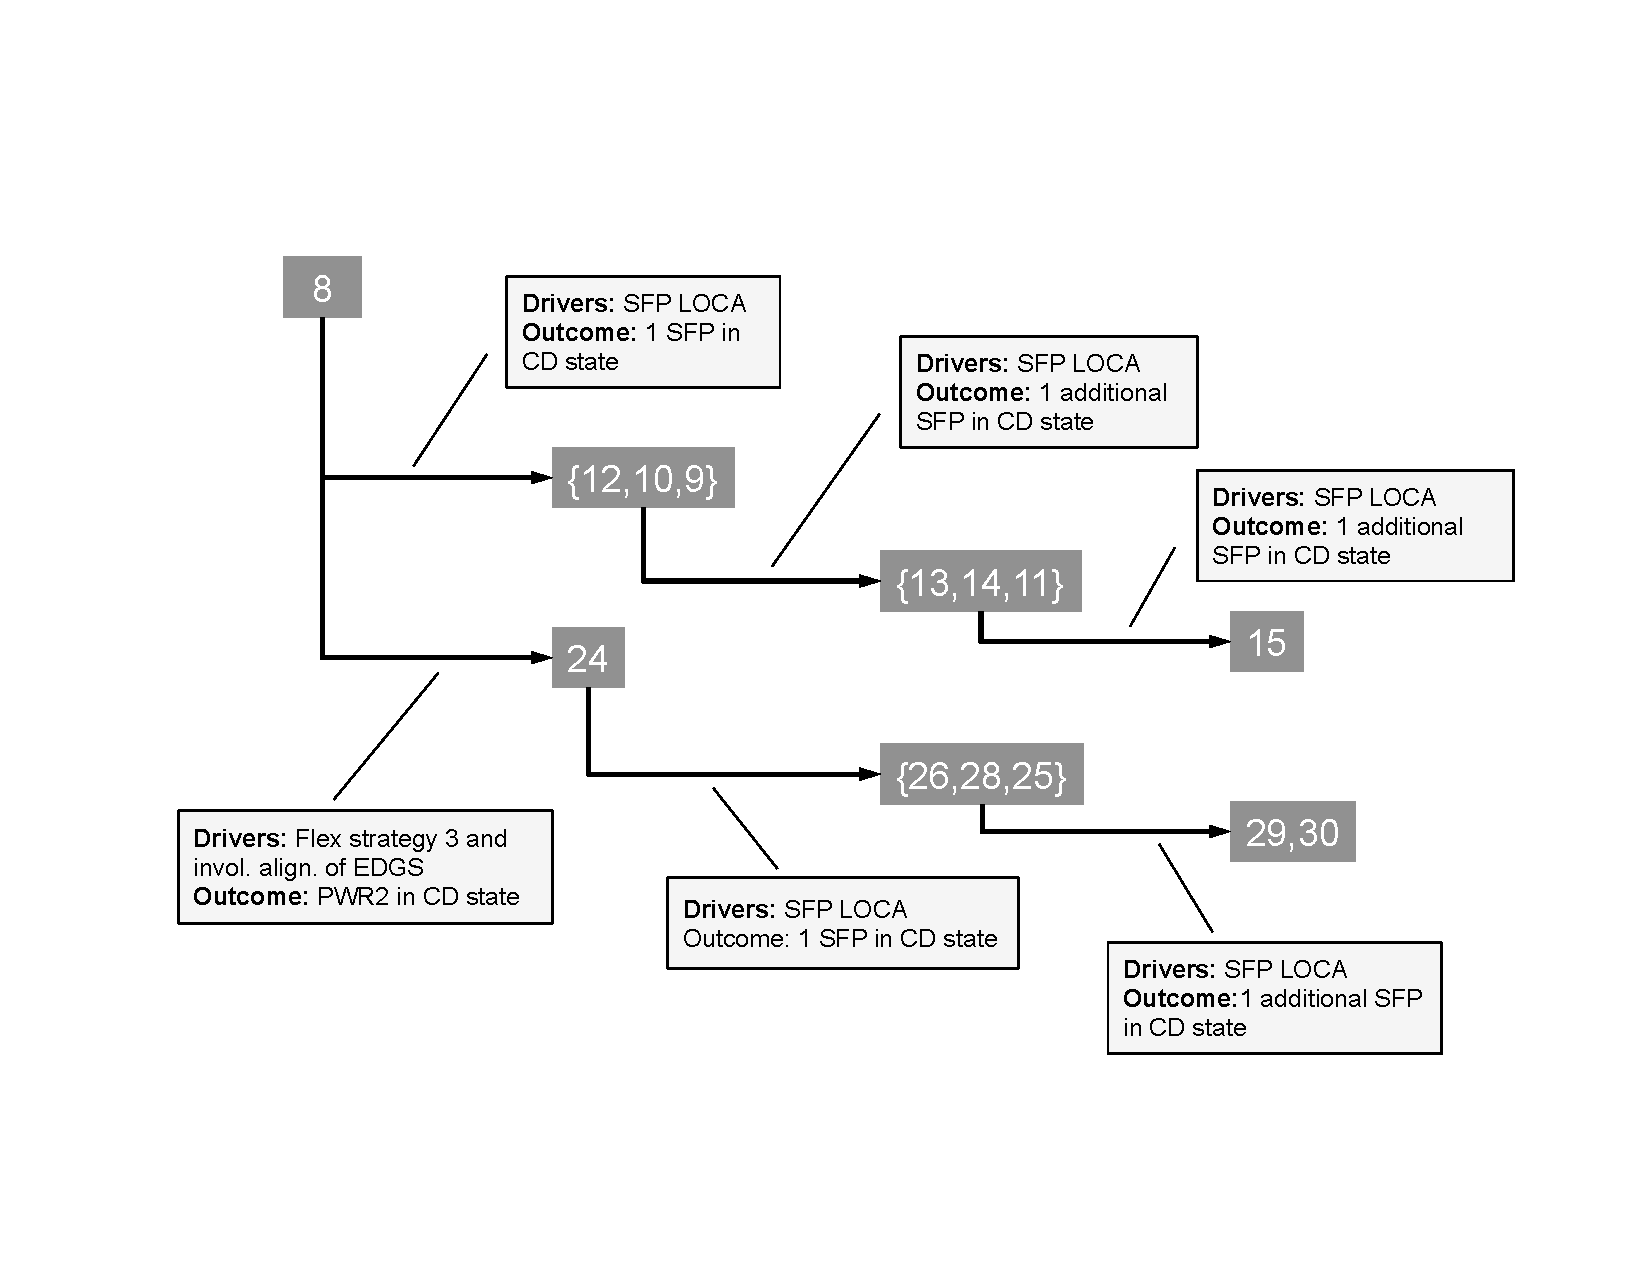
\includegraphics[scale=0.5]{PDSscheme.pdf}}
    \caption{Summary of the relationships among PDSs.}
    \label{fig:PDSsummary}
\end{figure}

\subsection{PDS8}
This PDS contains the majority of the data generated (about 890,000 samples fall in this category).
A first observation is about the SFPs: by looking at the histograms of the variable locaTime for each SFP
we see a drift of the histogram toward the highest bin (see Fig.~\ref{fig:histPDS8_8_locaTimeSFP}). 
The variable locaTimeSFP indicates when the actual LOCA
occurs: recall that locaTimeSFP=86400 implies LOCA does not occur.
Figure~\ref{fig:histPDS8_8_locaTimeSFP} implies that despite the presence of a 
loss of fluid in a SFP, it is possible to put the SFP in safe condition if certain conditions are met.

\begin{figure}
  \begin{subfigure}{.5\linewidth}
    \centering
    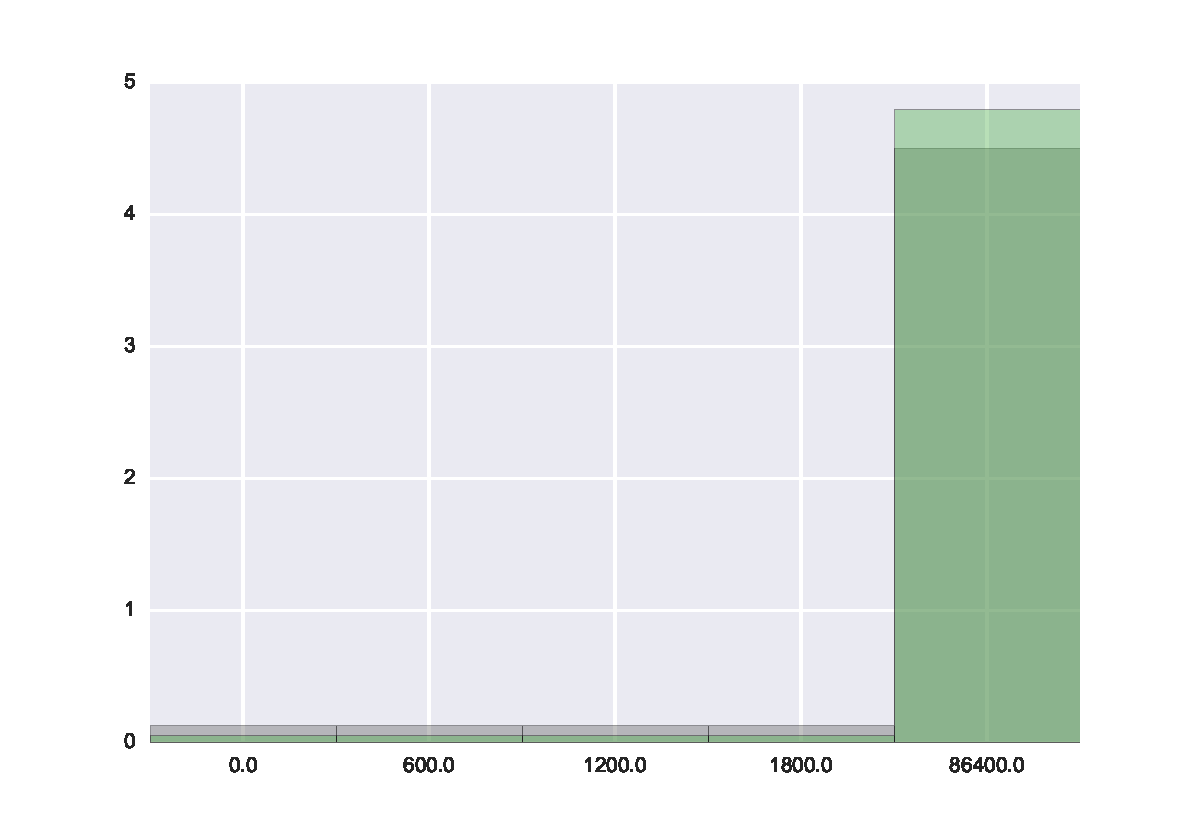
\includegraphics[scale=0.3]{8_locaTimeSFP1.pdf}
  \end{subfigure}%
  \begin{subfigure}{.5\linewidth}
    \centering
    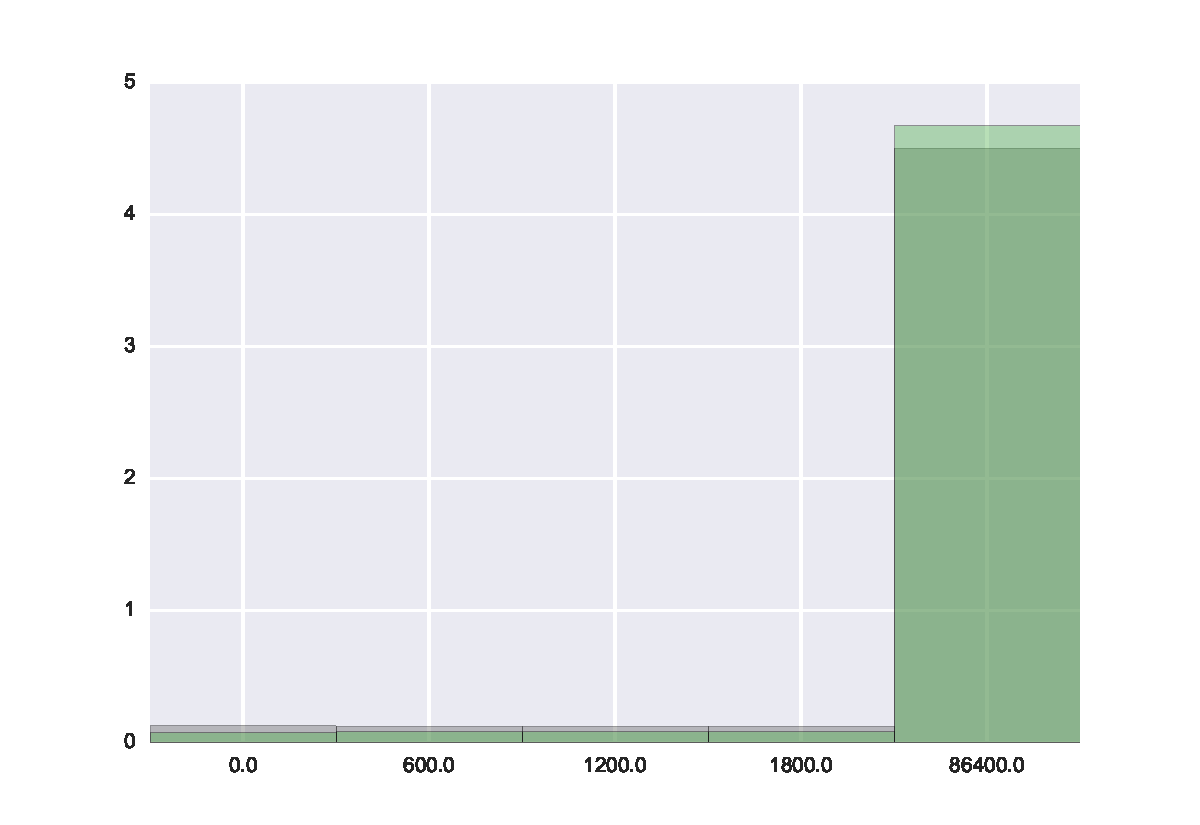
\includegraphics[scale=0.3]{8_locaTimeSFP2.pdf}
  \end{subfigure}\\[1ex]
  \begin{subfigure}{\linewidth}
    \centering
    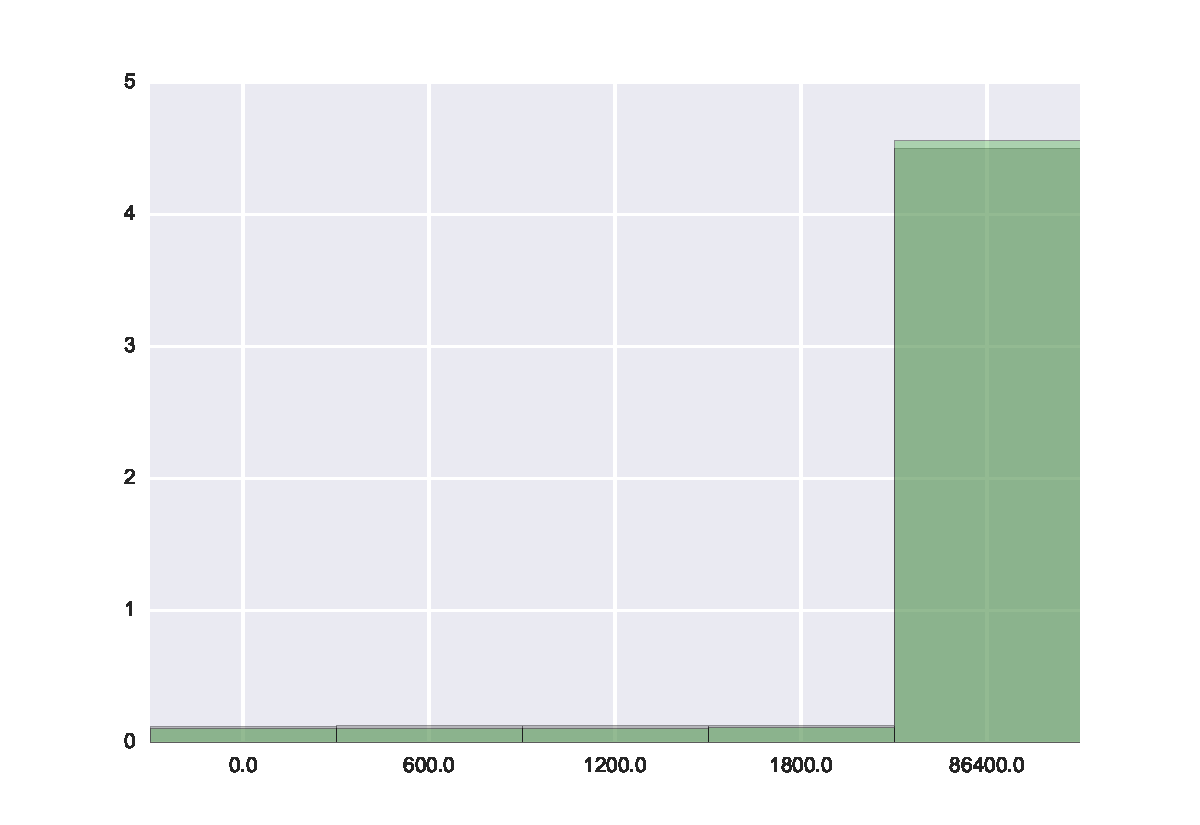
\includegraphics[scale=0.3]{8_locaTimeSFP3.pdf}
  \end{subfigure}
  \caption{PDS8: histograms of the variables locaTimeSFP1 (top left), locaTimeSFP2 (top right) and locaTimeSFP3 (bottom).}
  \label{fig:histPDS8_8_locaTimeSFP}
\end{figure}

The next step is to discover which are these conditions: this can be accomplished by considering the data samples
in PDS8 that actually have a SFP LOCA (i.e., samples characterized by locaTimeSFP2 different than 86400) 
and creating a scatter plot
in a 2-dimensional space where one dimension is the size of the SFP LOCA and the the second one is
the absolute time (i.e., the exact time) when the SFP is put in a safe state. 
Depending on the unit, this safe state can be reached in different ways:
\begin{itemize}
  \item Unit 1: when EDGS is aligned to Unit 1 or when EPE1 is connected to Unit 1
  \item Unit 2: when EPE2 is connected to Unit 2; note that the erroneous alignment of EDGS plays a role here since
                its occurrence brings it in an critical condition (no cooling in SFP)
  \item Unit 3: when EPE3 is connected to Unit 3
\end{itemize}

Figure~\ref{fig:scatterPDS8} shows four images; each image contains a scatter plot and an histogram along each 
dimension. Recall that all points in this scatter plots are characterized by SFP in an OK state.
From Fig.~\ref{fig:scatterPDS8} we can see the following:
\begin{itemize}
  \item Unit 1 (top left image): this scatter plot shows locaSizeSFP1 vs. SFP1 recovery time (which is represented 
        as the minimum value among EDGS is aligned to Unit 1) and EPE1 connected to Unit 1. Note that a SFP1 recovery 
        time less than 25,000 seconds (points on the left of the scatter plot) can recover a small SFP LOCA (i.e, 5.E-4). 
        Note also that a few points are clustered at around 12,000 seconds for SFP1 recovery time and a medium SFP LOCA (i.e., 3.5E-3). 
        This small group of points are characterized by the following distinctive features: recovery strategy 3, no EDGS erroneous 
        alignment and very early AC12 cross-tie (i.e., AC power of Unit 2 is provided to Unit 1 through a AC 
        cross-tie). This feature implies that even a medium SFP LOCA can be recovered only if recovery strategy 3 is
        chosen (see Fig.~\ref{fig:strategy3Scheme}) and, the AC cross-tie between Unit 2 and Unit 1 is completed 
        before 12,700 s. From this plot it can be observed that a large SFP LOCA can not be recovered.
  \item Unit 2 (top right and bottom left images): these two scatter plots shows similar thresholds for Unit 2. 
        Note two features: a large SFP LOCA can be recovered and the EDGS erroneous alignment impacts the threshold value 
        small and medium SFP LOCA.
  \item Unit 3 (bottom right image): since SFP3 as a higher heat load it is expected that the thresholds decrease. This
        is confirmed by comparing the bottom right scatter plot with the upper lefp plot of Fig.~\ref{fig:scatterPDS8}.
\end{itemize}


\begin{figure}
  \begin{subfigure}{.5\linewidth}
    \centering
    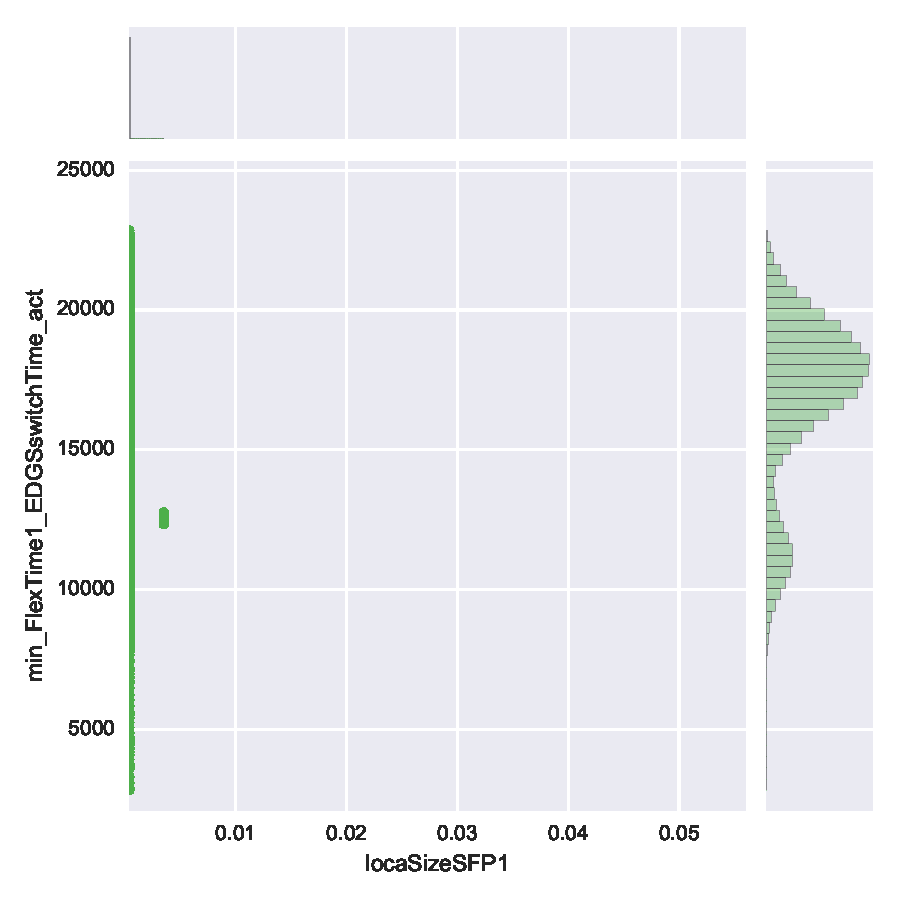
\includegraphics[scale=0.3]{8_sfp1_only_locaSizeSFP1_v_min_FlexTime1_EDGSswitchTime_act_scatter.pdf}
  \end{subfigure}%
  \begin{subfigure}{.5\linewidth}
    \centering
    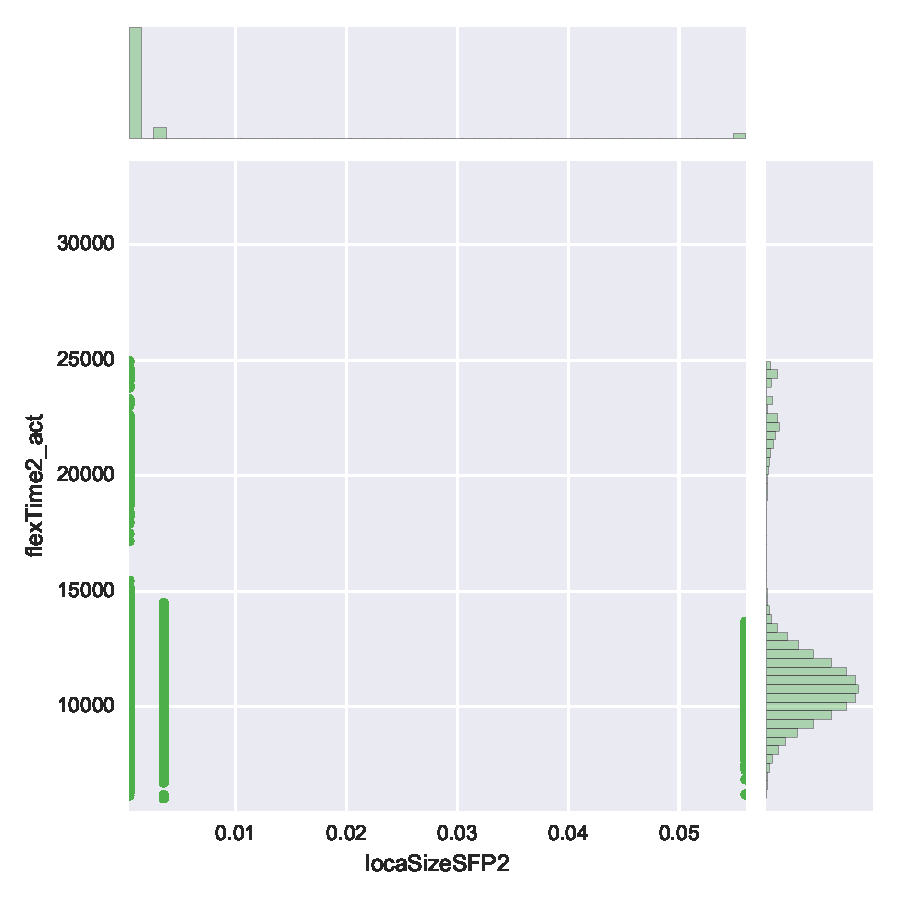
\includegraphics[scale=0.3]{8_sfp2_only_EDGSinvolAlign=0_locaSizeSFP2_v_flexTime2_act_scatter.pdf}
  \end{subfigure}\\[1ex]
  \begin{subfigure}{.5\linewidth}
    \centering
    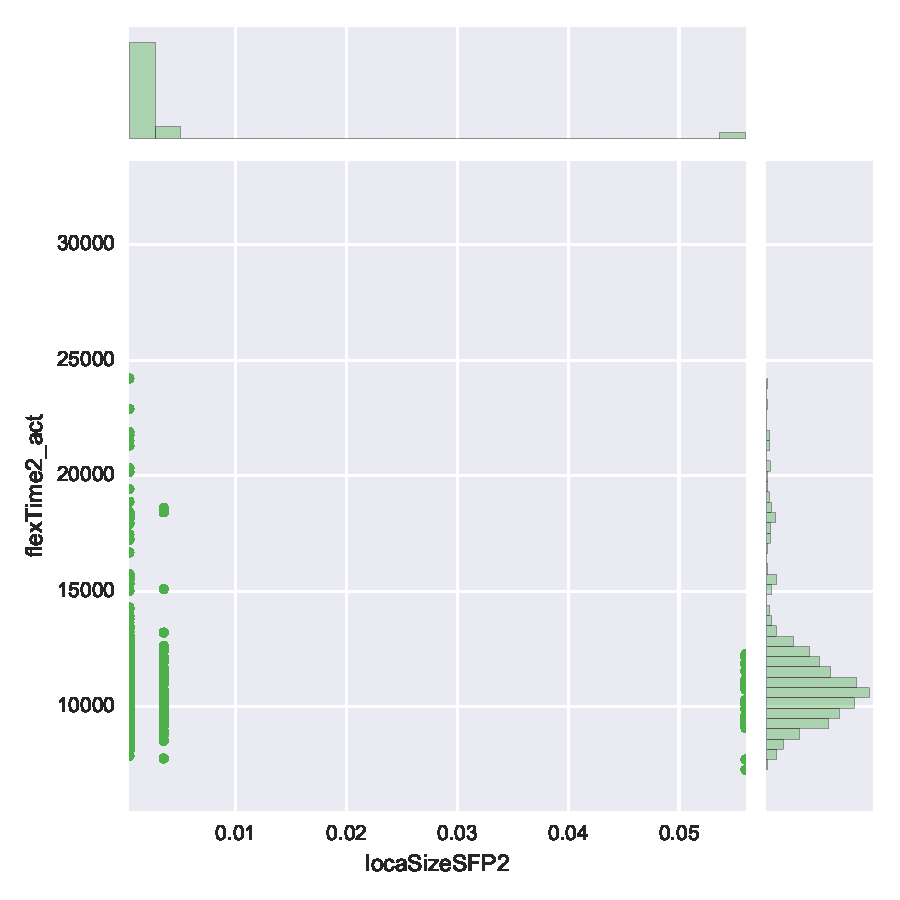
\includegraphics[scale=0.3]{8_sfp2_only_EDGSinvolAlign=1_locaSizeSFP2_v_flexTime2_act_scatter.pdf}
  \end{subfigure}
  \begin{subfigure}{.5\linewidth}
    \centering
    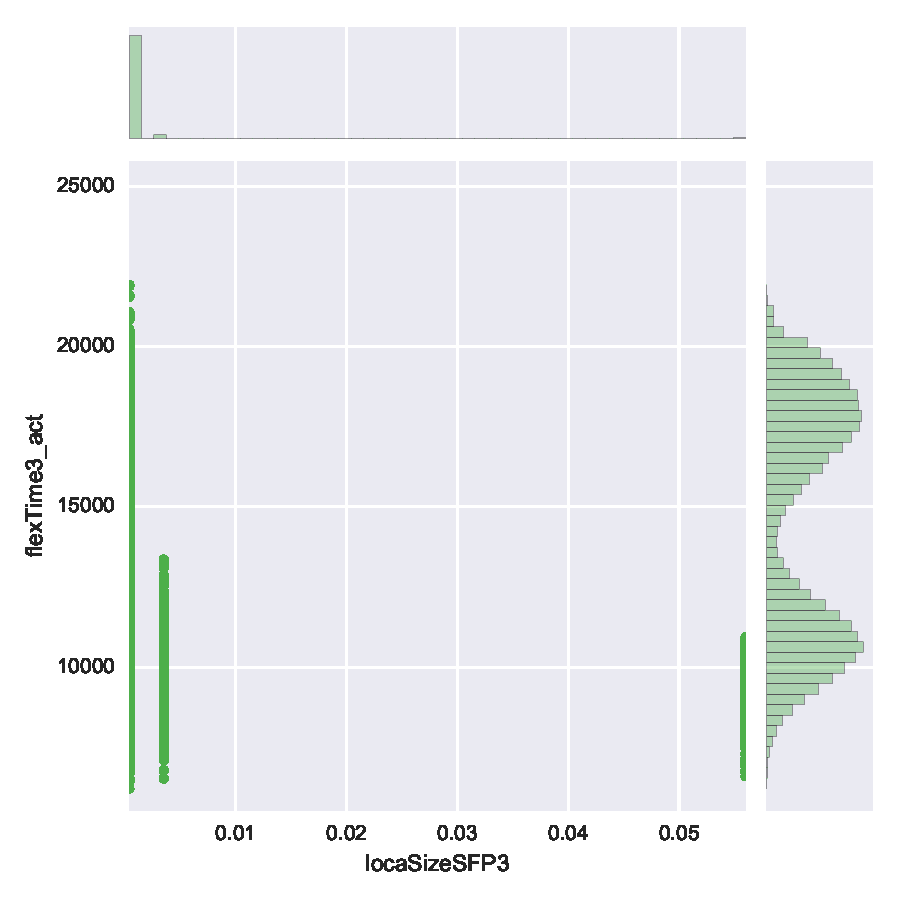
\includegraphics[scale=0.3]{8_sfp3_only_locaSizeSFP3_v_flexTime3_act_scatter.pdf}
  \end{subfigure}
  \caption{PDS8: scatter plot for SFP1 (top left), SFP2 with EDGS erroneous alignment (top right), 
           SFP2 without EDGS erroneous alignment (bottom right) and SFP3 (bottom right).}
  \label{fig:scatterPDS8}
\end{figure}  

\subsection{PDSs 12, 10, 9}
PDSs number 12, 10 and 9 are characterized by a single SFP in CD condition (on top of PWR3): SFP1, 
SFP2 and SFP3 respectively. The main driver is the loss of water inventory due to the seismic induced
SFP LOCA.
This conclusion might be obvious given the nature of the system; however, if we observe the 
histogram of the recovery strategy in each of these three PDSs 
(see Fig.~\ref{fig:histPDS_12_10_9_recoveryStrategy}) we observe a pattern.
PDS12 and PDS9 are dominated mainly by samples that follow Strategy 1 and 2 while PDS10 is 
exclusively characterized by simulations that followed Strategy 3.
This is due to the fact that unit prioritization allows to recover only the first SFP through EPEs. 
Heating-up of the SFP is so fast that does not allow for two consecutive 
EPE timings to occur.

\begin{figure}
  \begin{subfigure}{.5\linewidth}
    \centering
    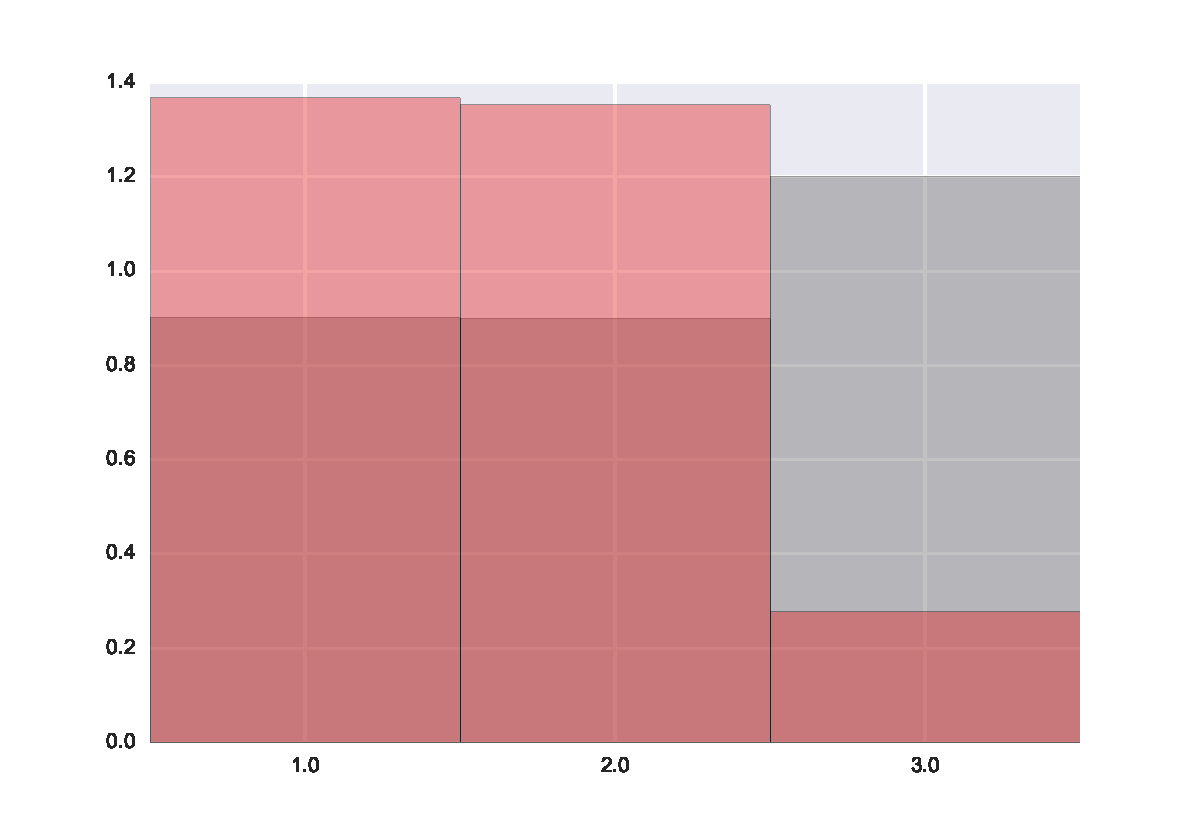
\includegraphics[scale=0.3]{12_recoveryStrategy.pdf}
  \end{subfigure}%
  \begin{subfigure}{.5\linewidth}
    \centering
    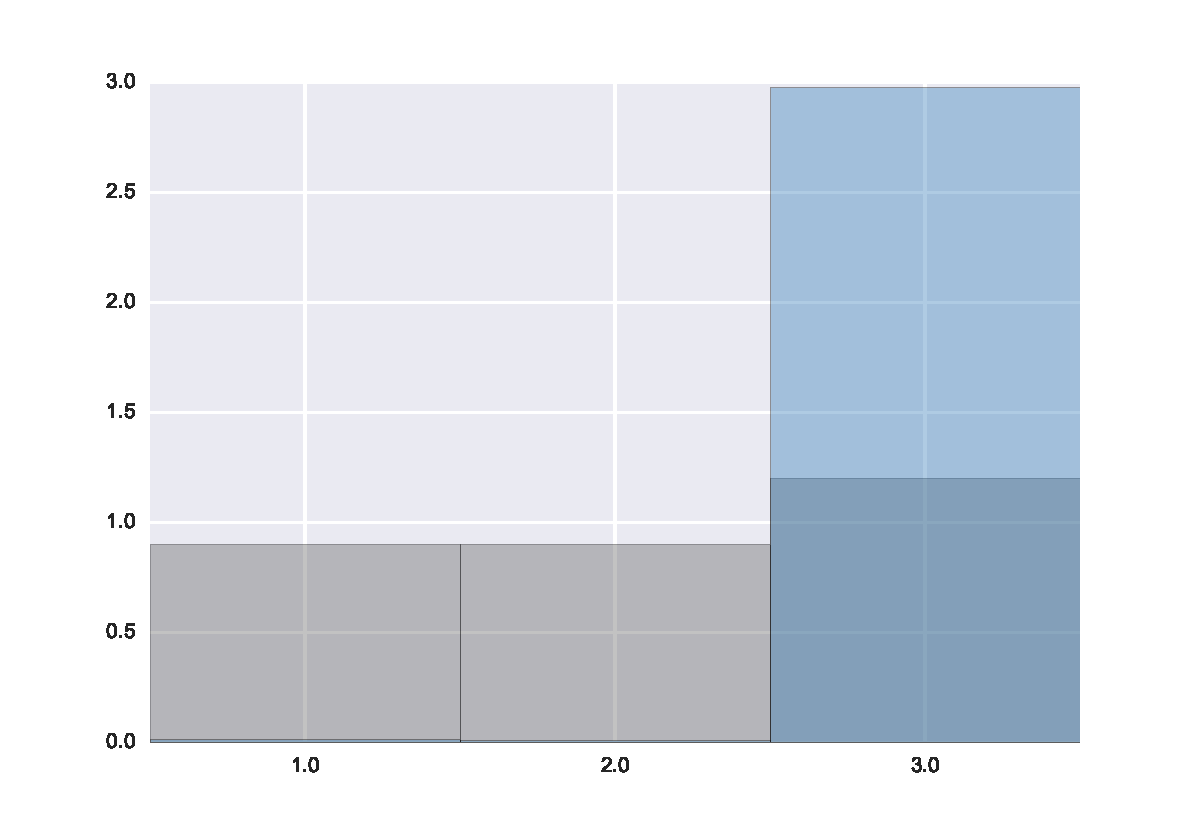
\includegraphics[scale=0.3]{10_recoveryStrategy.pdf}
  \end{subfigure}\\[1ex]
  \begin{subfigure}{\linewidth}
    \centering
    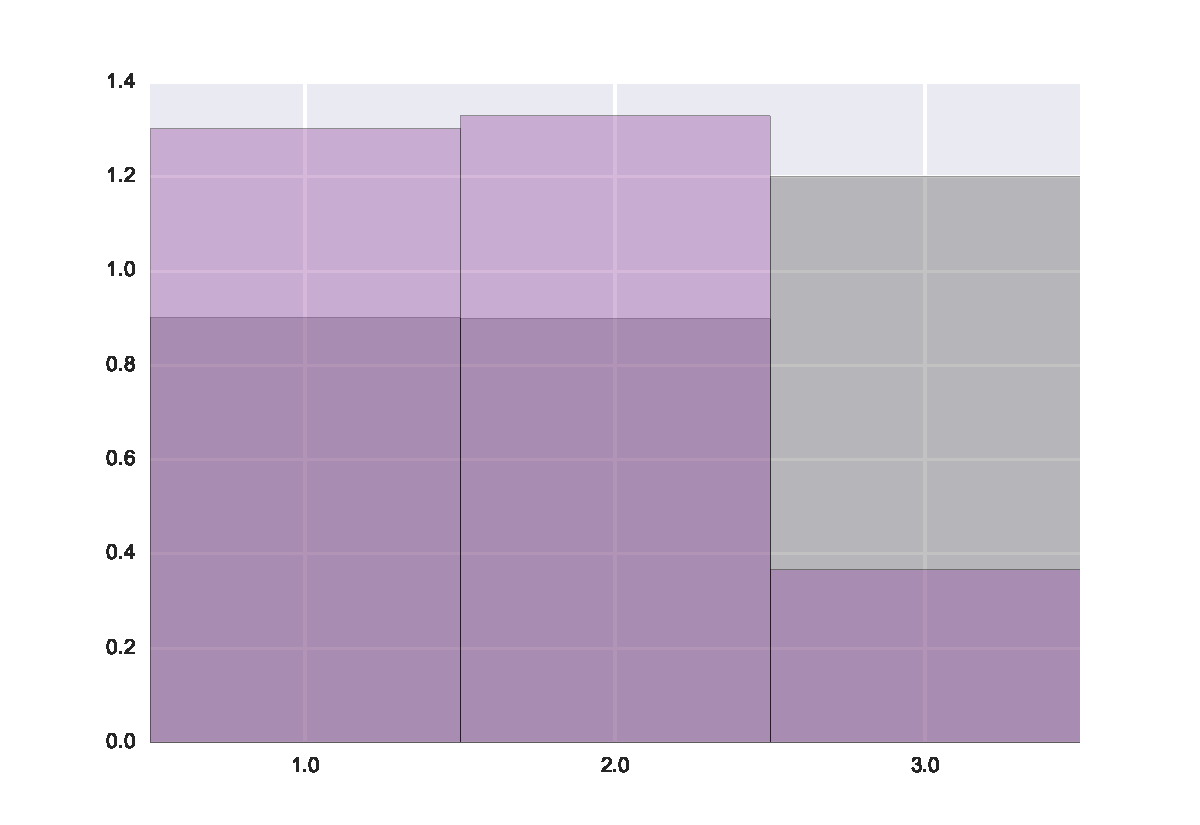
\includegraphics[scale=0.3]{9_recoveryStrategy.pdf}
  \end{subfigure}
  \caption{Histograms of the variable recovery strategy for PDS12 (top left), PDS10 (top right) and PDS9 (bottom)}
  \label{fig:histPDS_12_10_9_recoveryStrategy}
\end{figure}

\subsection{PDS24}
PDS24 is the first PDS that characterize an additional PWR to reach CD (on top of PWR3): PWR2. By looking at the
histogram of the input parameters (see Fig.~\ref{fig:histPDS_24}) that belong to this PDS we have identified 
that PWR2 reaches CD only if recovery strategy 3 is chosen. 
In addition, erroneous alignment of EDGS plays the major driver to reach PDS24. Interestingly, the time of such 
switch is also important: by looking at bottom histogram Fig.~\ref{fig:histPDS_24}, the distribution of the 
variable EDGSerrAlignTime is characterized by two modes, an early mode and a late mode.
This feature is due to the fact that, in strategy 3, EDGS erroneous alignment 
(see Fig.~\ref{fig:strategy3SchemeInvolAlign}) might run in parallel with EPE3 or EPE1.
If this erroneous action occurs when EPE3 or EPE1 have just started, then PWR2 reaches CD almost certainly due to
the PWR2 heat-up. If this erroneous action occurs when EPE3 or EPE1 are almost completed, then the EPE team
has time to prioritize Unit 2 and quickly recovery it.
The two modes of the bottom histogram of Fig.~\ref{fig:histPDS_24} correspond to an EDGS 
erroneous action that occurs right after EPE operation for Unit 3 (early mode) and for Unit 1 (late mode) has 
started.

\begin{figure}
  \begin{subfigure}{.5\linewidth}
    \centering
    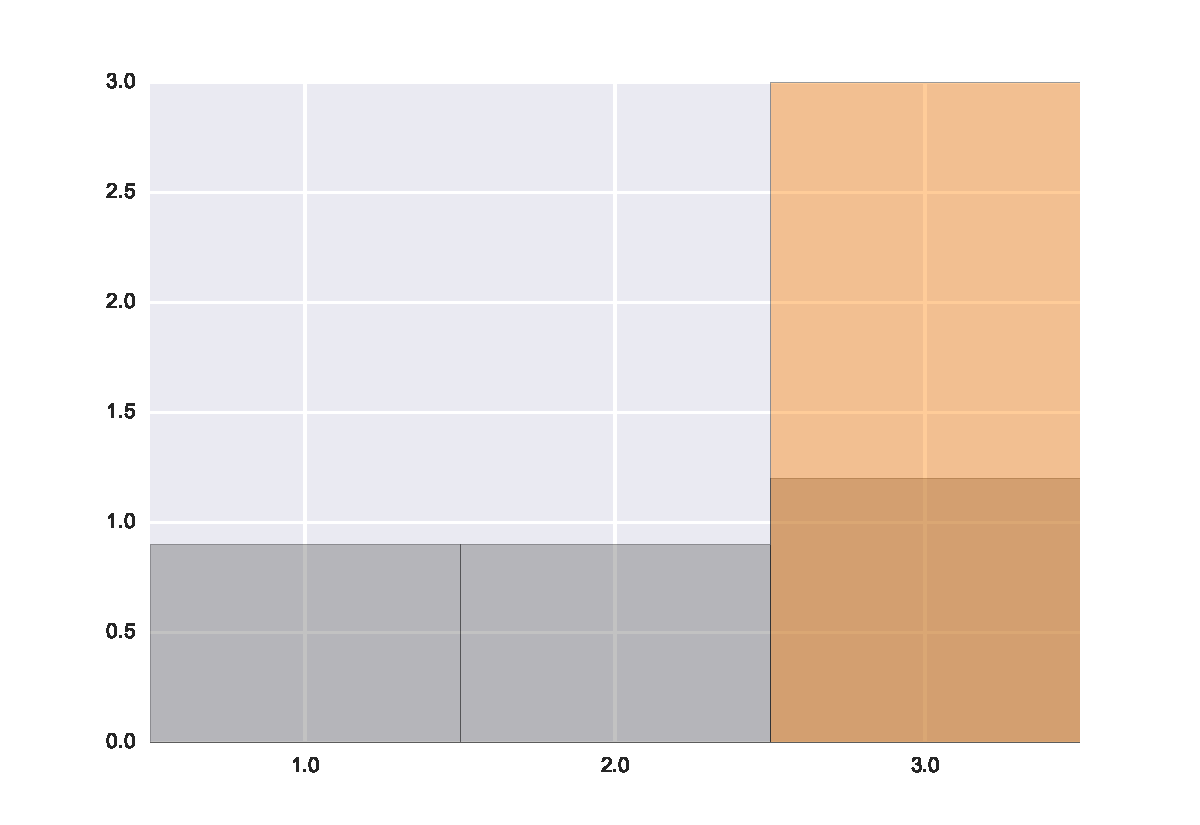
\includegraphics[scale=0.3]{24_recoveryStrategy.pdf}
  \end{subfigure}%
  \begin{subfigure}{.5\linewidth}
    \centering
    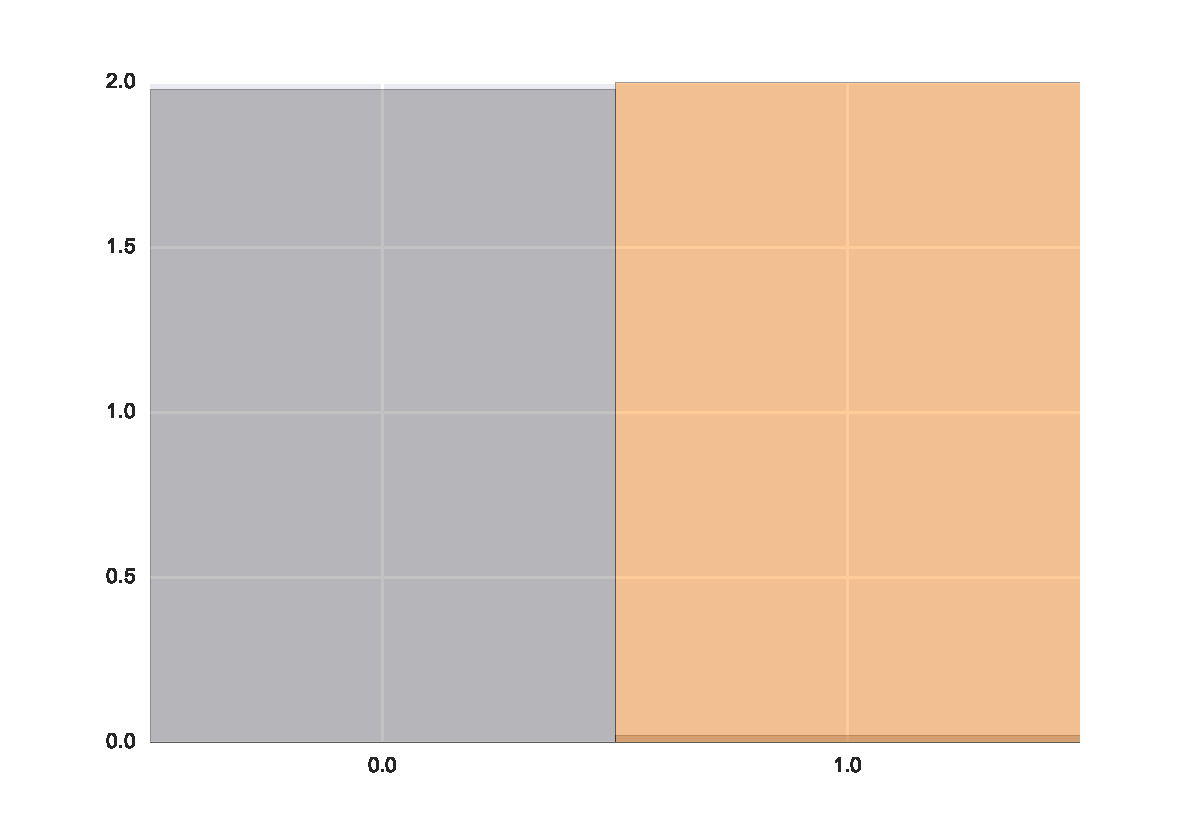
\includegraphics[scale=0.3]{24_EDGSinvolAlign.pdf}
  \end{subfigure}\\[1ex]
  \begin{subfigure}{\linewidth}
    \centering
    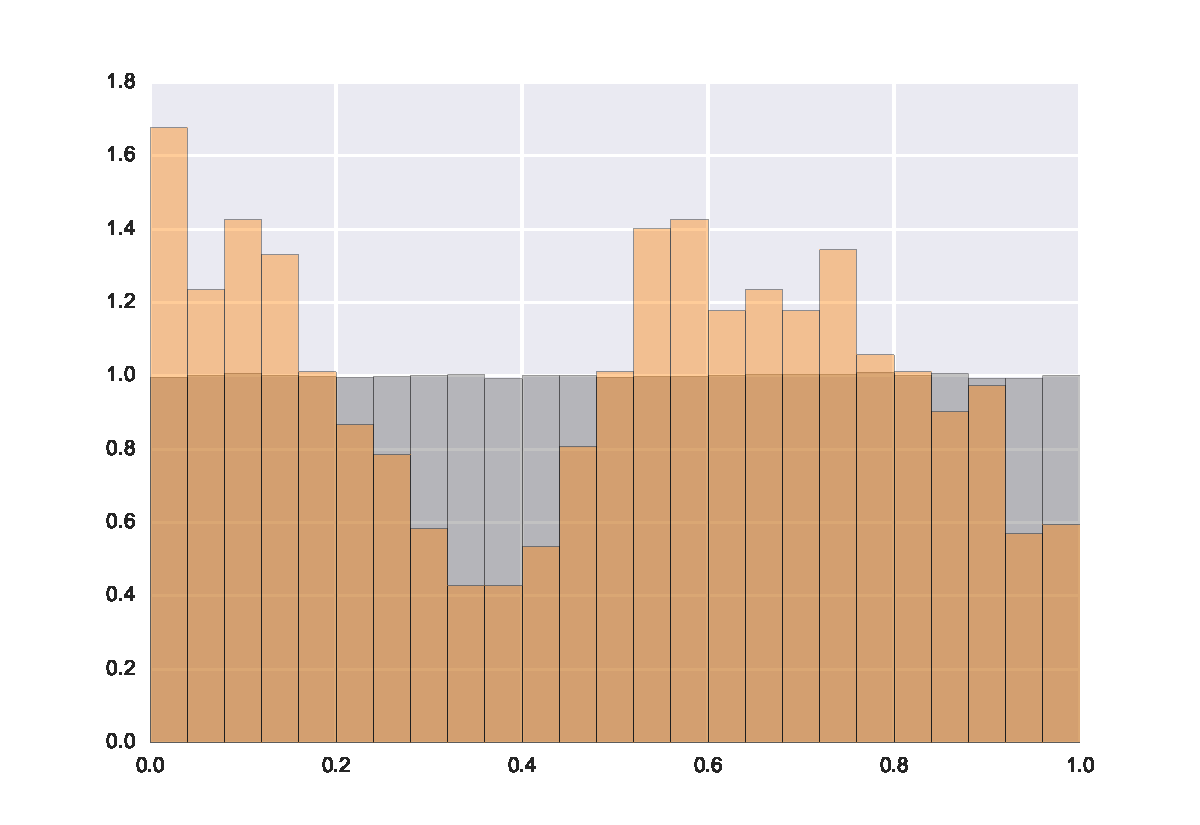
\includegraphics[scale=0.3]{24_EDGSinvolAlignTime.pdf}
  \end{subfigure}
  \caption{PDS24: histograms of the variables recovery (top left), EDGSerrAlign (top right) and EDGSerrAlignTime (bottom)}
  \label{fig:histPDS_24}
\end{figure}

\subsection{PDSs 13, 14, 11}
PDSs 13, 14 and 11 is a blend of PDS 12, 10 and 9: they contains 2 SFPs in CD condition (in addition to PWR3). 
hese PDS can be simply characterized
by the occurrence of 2 SFP LOCAs which are not correlated events; i.e., SFP LOCA have been modeled as independent events.
Thus, the same conclusions derived from PDSs 9, 10 and 12, can be transposed for PDSs 13, 14 and 11.

\subsection{PDSs 26, 28, 25}
PDSs 26, 28 and 25 are characterized by 1 SFP along with PWR2 and PWR3 in CD condition; thus it 
represents a mix of PDS 24 and PDS 12, 10 and 9.
These PDS are in fact characterized by recovery strategy 3 and EDGS erroneous align along with a SFP LOCA.
Similarly to what has been presented for PDS24, the interesting histogram of EDGS erroneous time for 
these three PDSs (see Fig.~\ref{fig:histPDS_26_28_25_EDGSinvolAlignTime}). Note these histograms follow the same pattern 
of Fig.~\ref{fig:histPDS_24} (bottom plot).

\begin{figure}
  \begin{subfigure}{.5\linewidth}
    \centering
    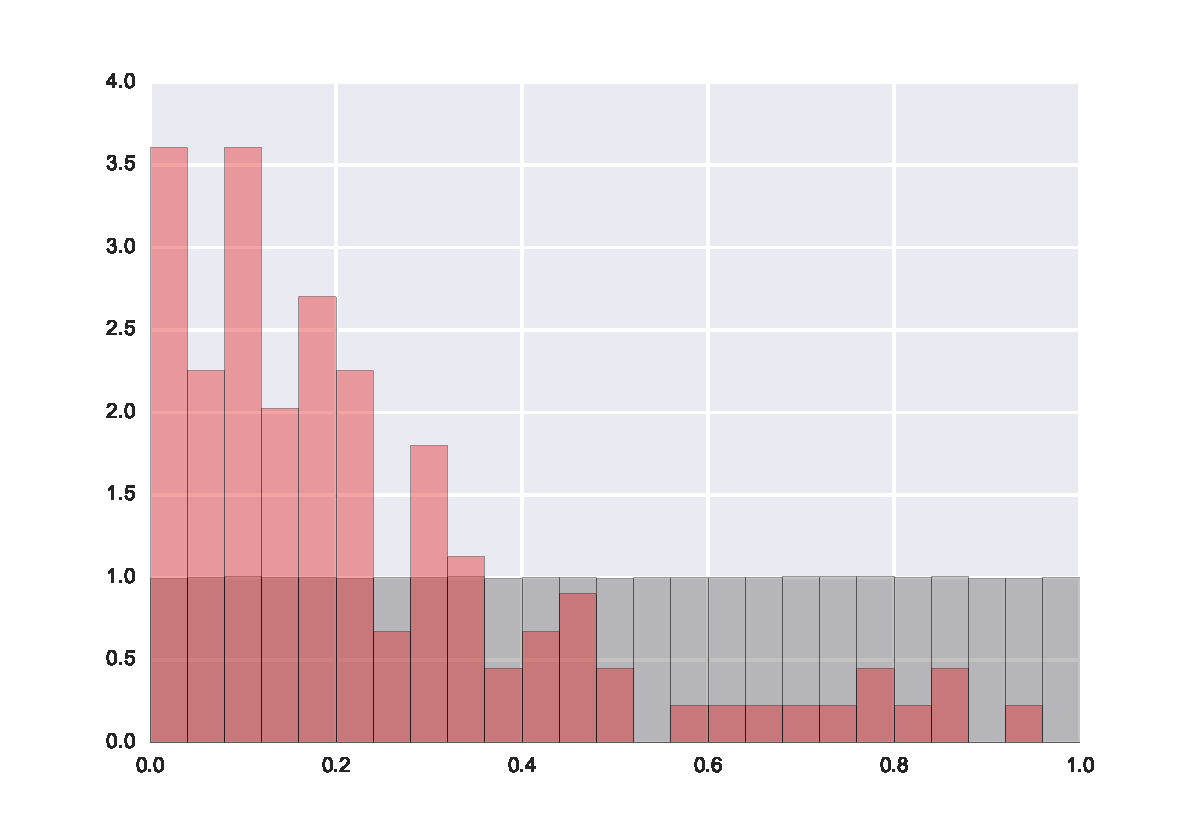
\includegraphics[scale=0.3]{28_EDGSinvolAlignTime.pdf}
  \end{subfigure}%
  \begin{subfigure}{.5\linewidth}
    \centering
    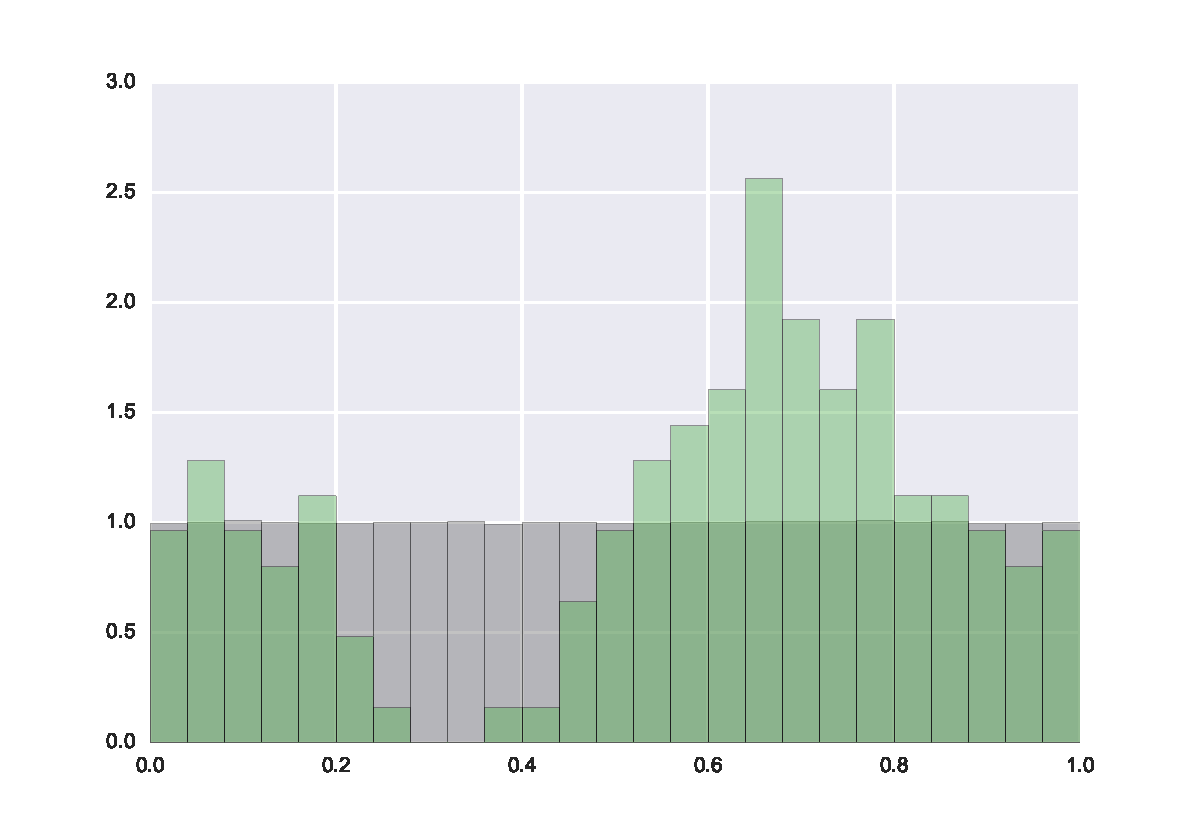
\includegraphics[scale=0.3]{26_EDGSinvolAlignTime.pdf}
  \end{subfigure}\\[1ex]
  \begin{subfigure}{\linewidth}
    \centering
    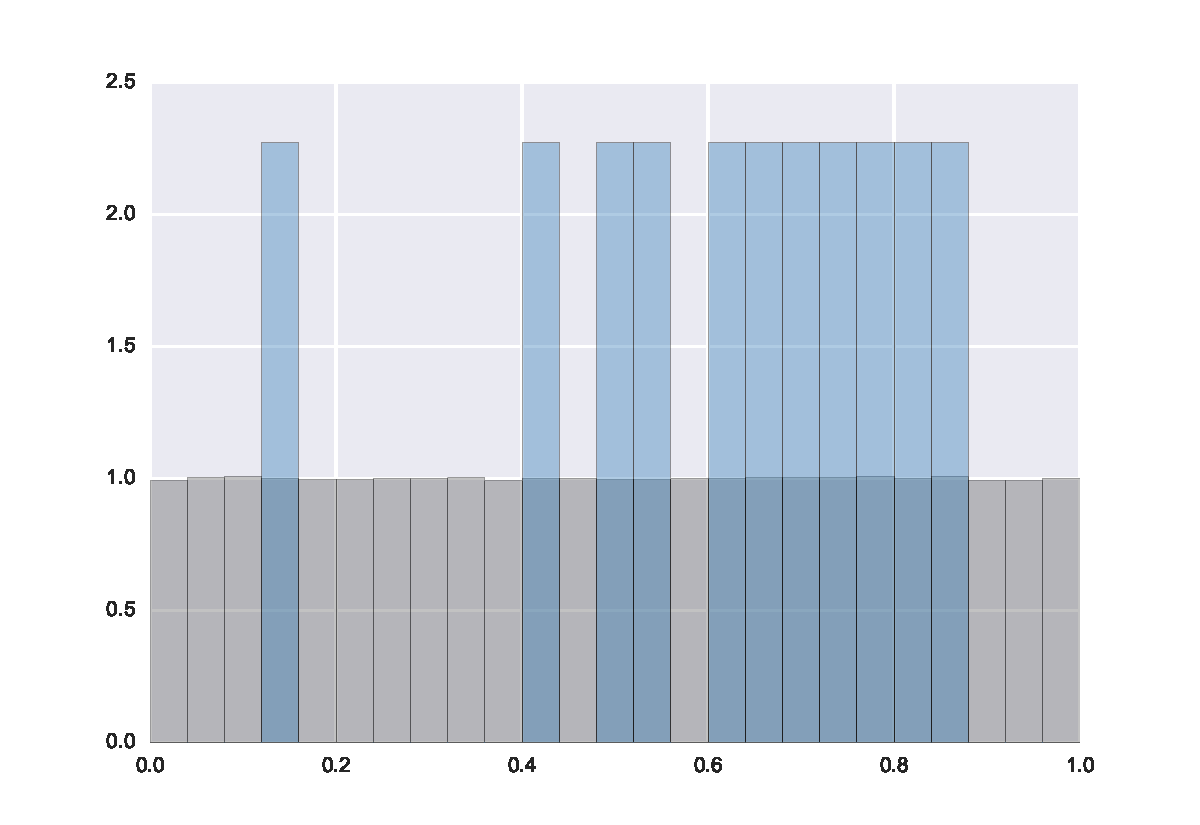
\includegraphics[scale=0.3]{25_EDGSinvolAlignTime.pdf}
  \end{subfigure}
  \caption{Histograms of the variable EDGSerrAlignTime for PDS28 (top left), PDS26 (top right) and PDS25 (bottom)}
  \label{fig:histPDS_26_28_25_EDGSinvolAlignTime}
\end{figure}

\subsection{PDS15}
PDS15 is characterized by having all SFPs in a CD state (along with PWR2). Similar to the considerations 
presented for PDSs 12, 10 and 9 (and also
similar to PDSs PDSs 13, 14, 11), the main driver is a medium/large LOCA for all SFPs coupled with long EPE time.

